\chapter*{Pitch perception - JND}
%
The purpose of this study is to evaluate the differential threshold, known as Just Noticeable Difference (JND), of pitch perception. Webers law states that the smallest detectable change in perception, \textit{$\Delta$I}, is equal to a constant, \textit{k}, times the physical stimulus intensity, \textit{I}. 
%
\begin{equation}
\Delta I = k \cdot I
\end{equation}
%
The constant, \textit{k}, is known as the Weber Fraction for a particular sensory dimension.
%

\section*{Methods}
%
The psychometric method used for stimuli presentation is the Method of Constant Stimuli which prescribe that the experimenter chooses a number of stimulus intensities and a reference intensity. In this study the stimulus intensity refers to frequency and the test subject reports which of the two stimuli are highest in pitch. The response is presented as a psychometric function. 

The chosen frequencies have to be a qualified guess about where the test subjects differential threshold is. In our study we base the qualified guess on the differential threshold found by \citet{Wier1977} at 800 Hz which is approximately 1.2 Hz. It is important that the intensity range covers intensities above and below the actual differential threshold so there must be stimuli which the test subject always report the correct answer to and vice versa. Based on a pilot test the intensity range was expanded with higher frequency differences because some of the test subjects did not reach a plateau of 100 \% correct answers. Based on the differential threshold approximation from \citet{Wier1977} and the pilot test, the intensity range consists of frequencies with a logarithmic difference from 800 Hz starting from 0.15 Hz to 76.8 Hz. Each frequency is repeated 10 times which leads to a total of 100 trials per test subject.  

Data collections is done by Two-Alternative Forced Choice (2-AFC). A more objective measure is obtained with 2-AFC because the test subjects are forced to make an answer whether or not they actually heard a difference between the two stimuli \citep[p. 1219]{Ehrenstein1999}. 2-AFC accounts for criterium biases when using multiple test subjects who might have different response criteria when answering which of the two frequency had the highest pitch. Criterium biases are avoided because the test subjects are forced to answer,  whether or not they have perceived a difference. When using this method there is a 50 \% chance of guessing which of the two stimuli had the highest pitch and therefore the JND is found where 75 \% of the answers are correct.\\[5mm]
%
In contrast to the two other classical psychometric methods the Method of Constant Stimuli prescribes randomization of stimuli representation which eliminates anticipation and habituation \citep[p. 15]{Poulsen2005}. One disadvantage with Method of Constant Stimuli is the measurement time. Each added repetition or stimulus intensity will add extra time in which the subjects must focus on pitch differences. This prolonged measurement time might lead to fatigue and risk of an altered differential threshold \citep[p. 16]{Poulsen2005}. 
%

\subsection*{Experimental setup}
%
The equipment used for the study is a pair of Bang $\&$ Olufsen H6 headphones, a Lenovo Thinkpad with a fixed 10 \% volume, and a programme (TwoAFC\_pitch) running in MatLab for stimuli presentation. The two tones are presented as A and B on the screen and the test subject has to choose the one they perceive as having the highest pitch by pressing one of the buttons accordingly. The experiment was conducted in a group room located on the 1st floor of Fredrik Bajers vej 7B, B2-207. \autoref{fig:experiment} illustrates the experimental setup.
%
\begin{figure}[H]
\centering
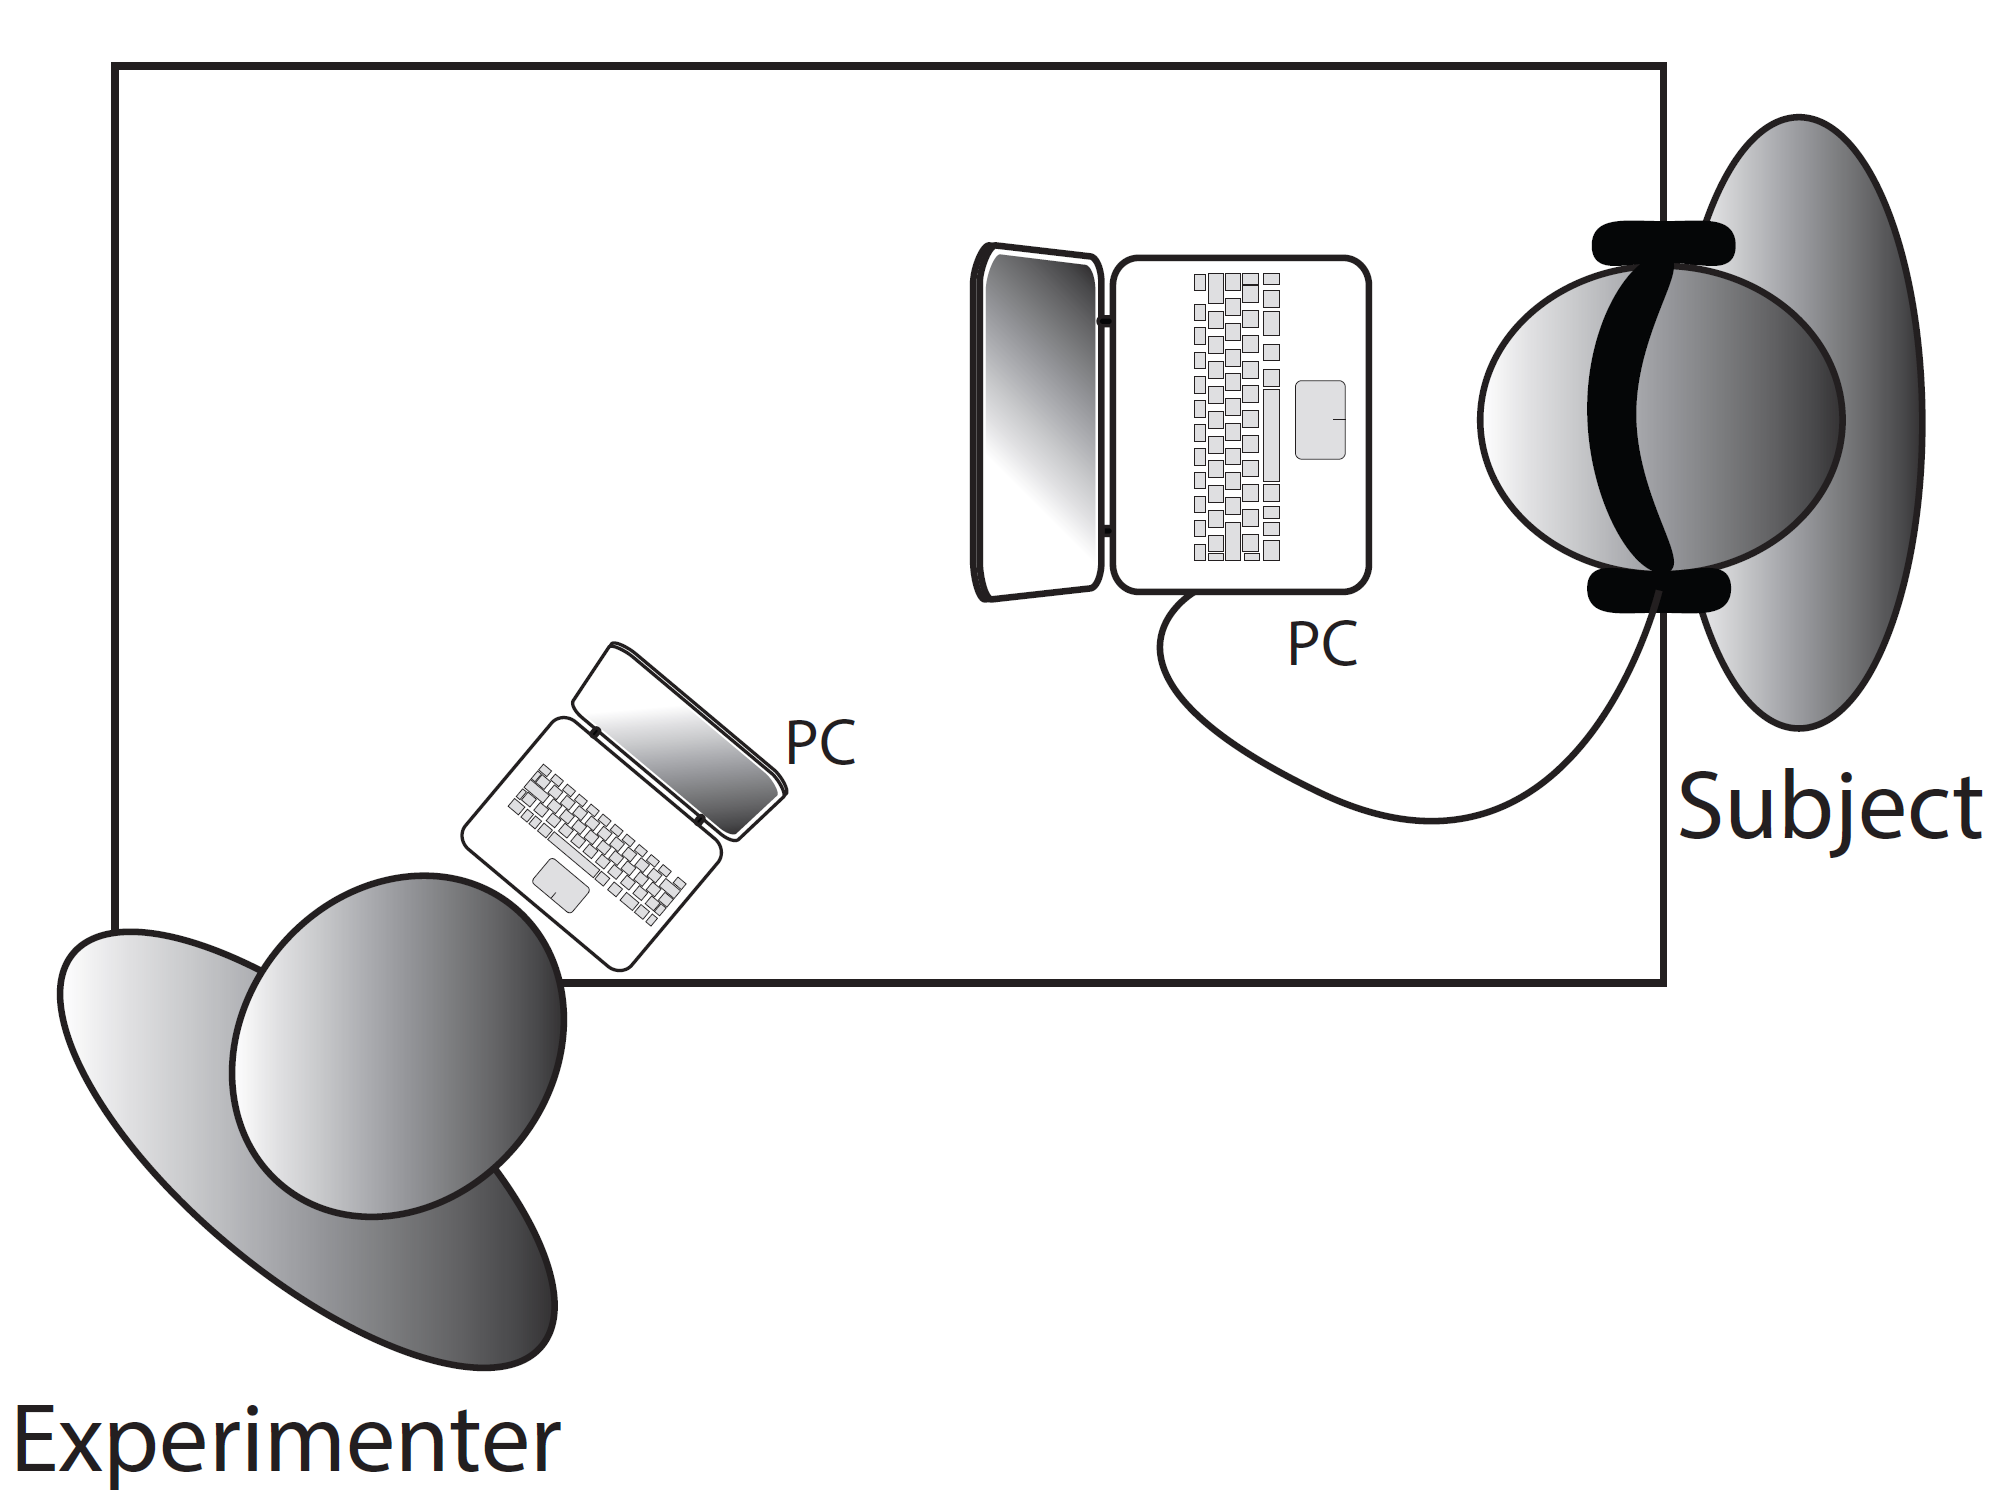
\includegraphics[width = 0.5\textwidth]{Figure/Vores_Figurer/experiment.png} 
\caption{A sketch of the experimental setup}
\label{fig:experiment}
\end{figure}
%

\subsection*{Test subjects}
%
Five test subjects were used in the test including two males and three females in the age of 23 to 24 (mean = 23.4). All of which are Engineering Psychology students at Aalborg University.

\subsection*{Pilot test}
%
Based on a pilot test it is decided to expand the stimuli intensity range down to 0.15 Hz and up to 76.8 Hz from the original range of intensities 0.3 Hz, 0.6 Hz, 1.2 Hz, 2.4 Hz, 4.8 Hz, 9.6 Hz. This is done because the female test subjects had problems detecting any difference in pitch even at the highest frequency differences.

\section*{Results}
%
On \autoref{fig:Subject1}, \autoref{fig:Subject2}, \autoref{fig:Subject3}, \autoref{fig:Subject4}, and \autoref{fig:Subject5} data from each test subject is presented along with the psychometric function. The response from the subjects are represented as the percentage of correct answers to each frequency difference, $\Delta$f.
% 
\begin{figure}[htb]
\centering
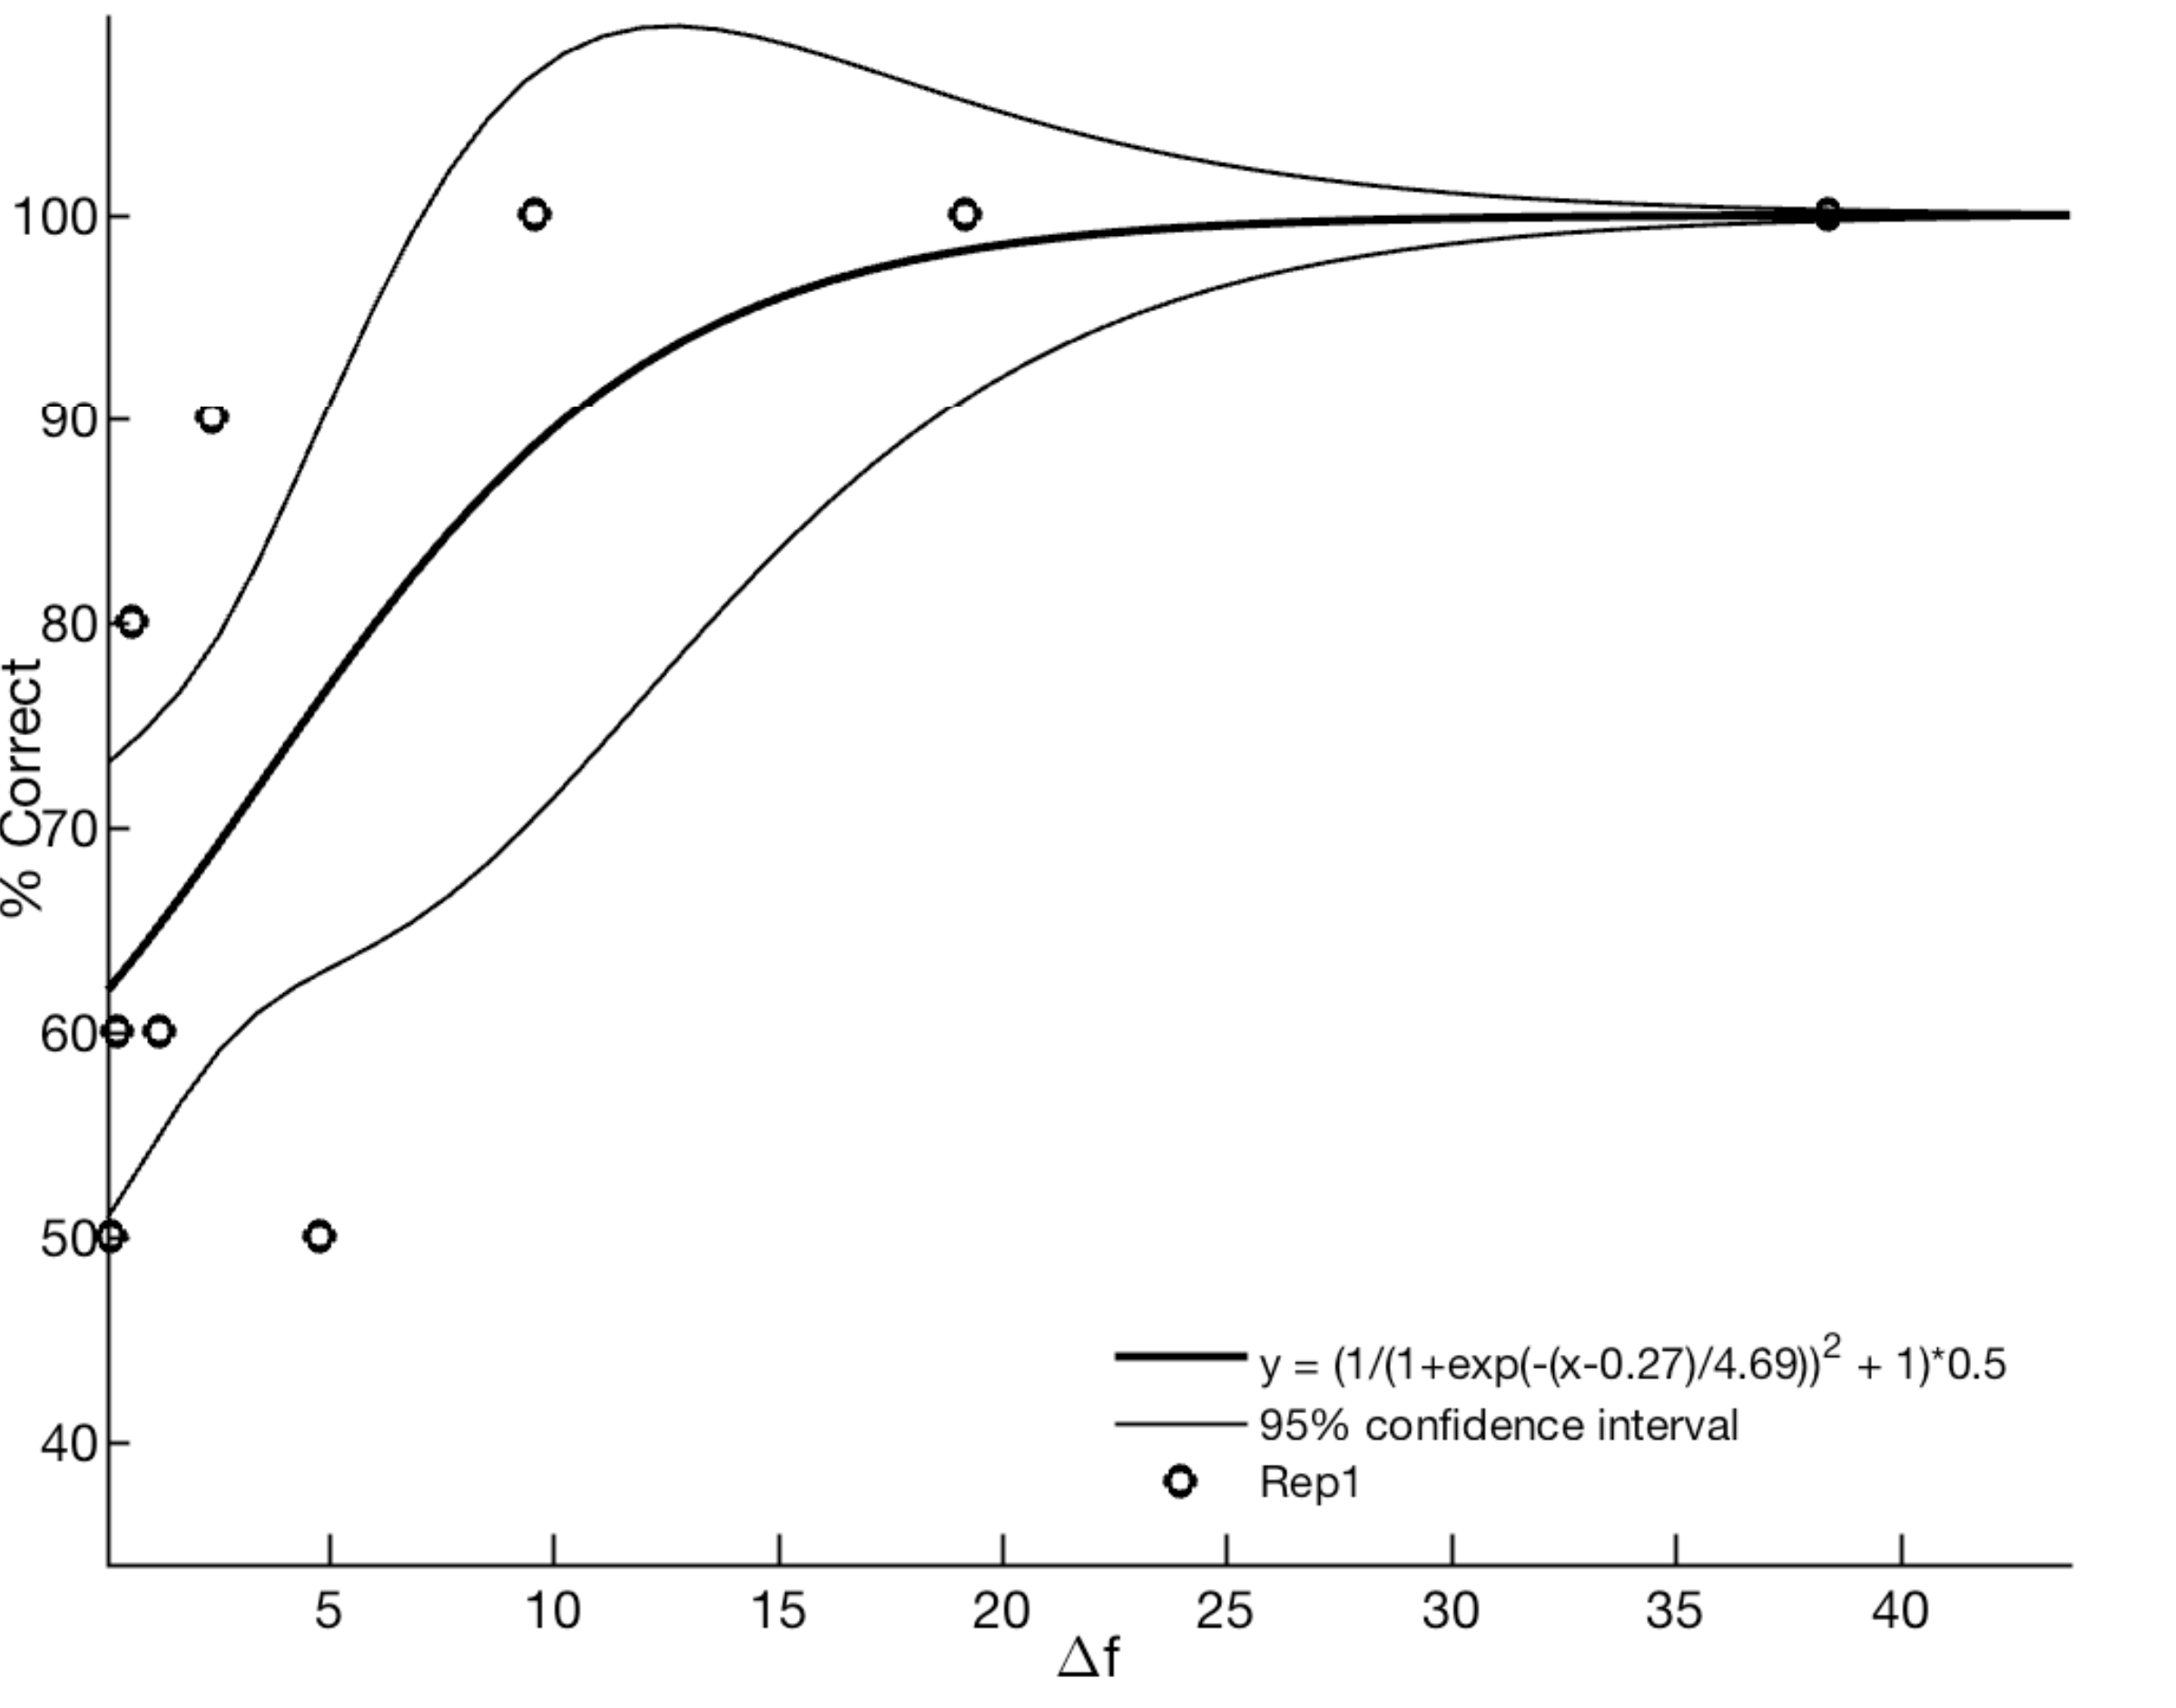
\includegraphics[width = 0.7\textwidth]{Figure/Vores_Figurer/Subject1.png} 
\caption{Raw data and fitted psychometric function for Subject 1.}
\label{fig:Subject1}
\end{figure}
%
\begin{figure}[htb]
\centering
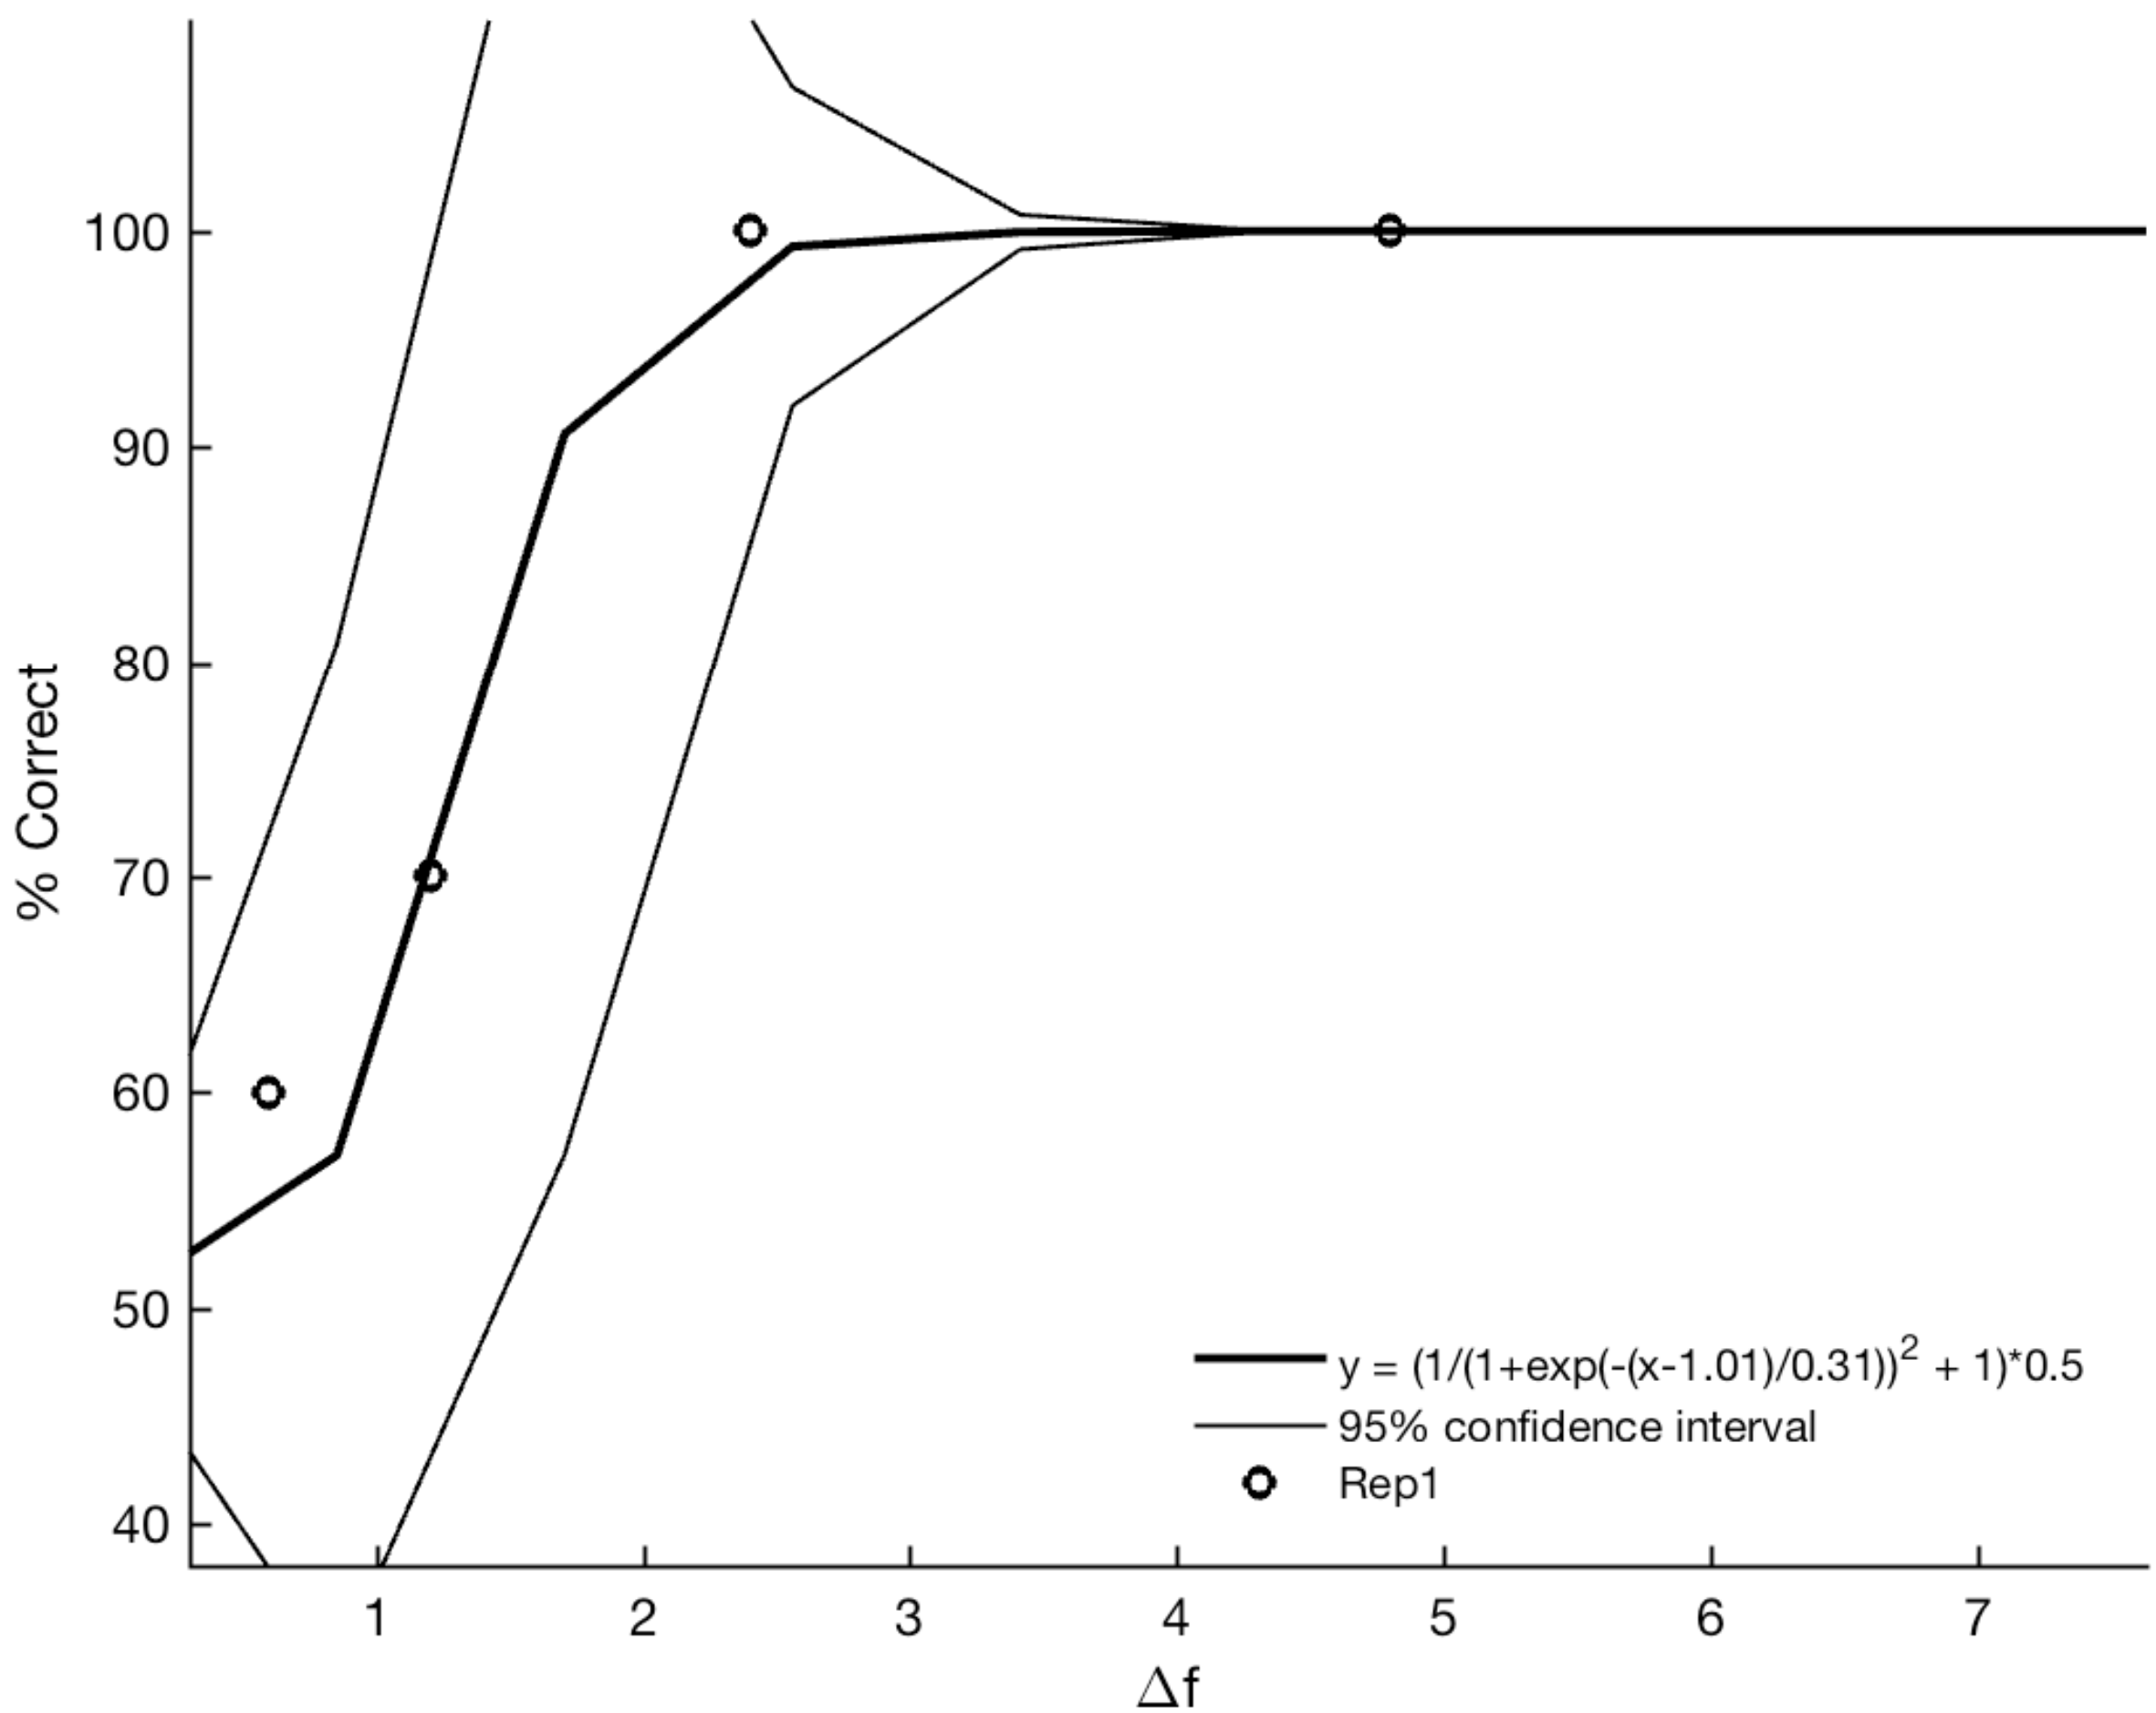
\includegraphics[width = 0.7\textwidth]{Figure/Vores_Figurer/Subject2.png} 
\caption{Raw data and fitted psychometric function for Subject 2.}
\label{fig:Subject2}
\end{figure}
%
\begin{figure}[htb]
\centering
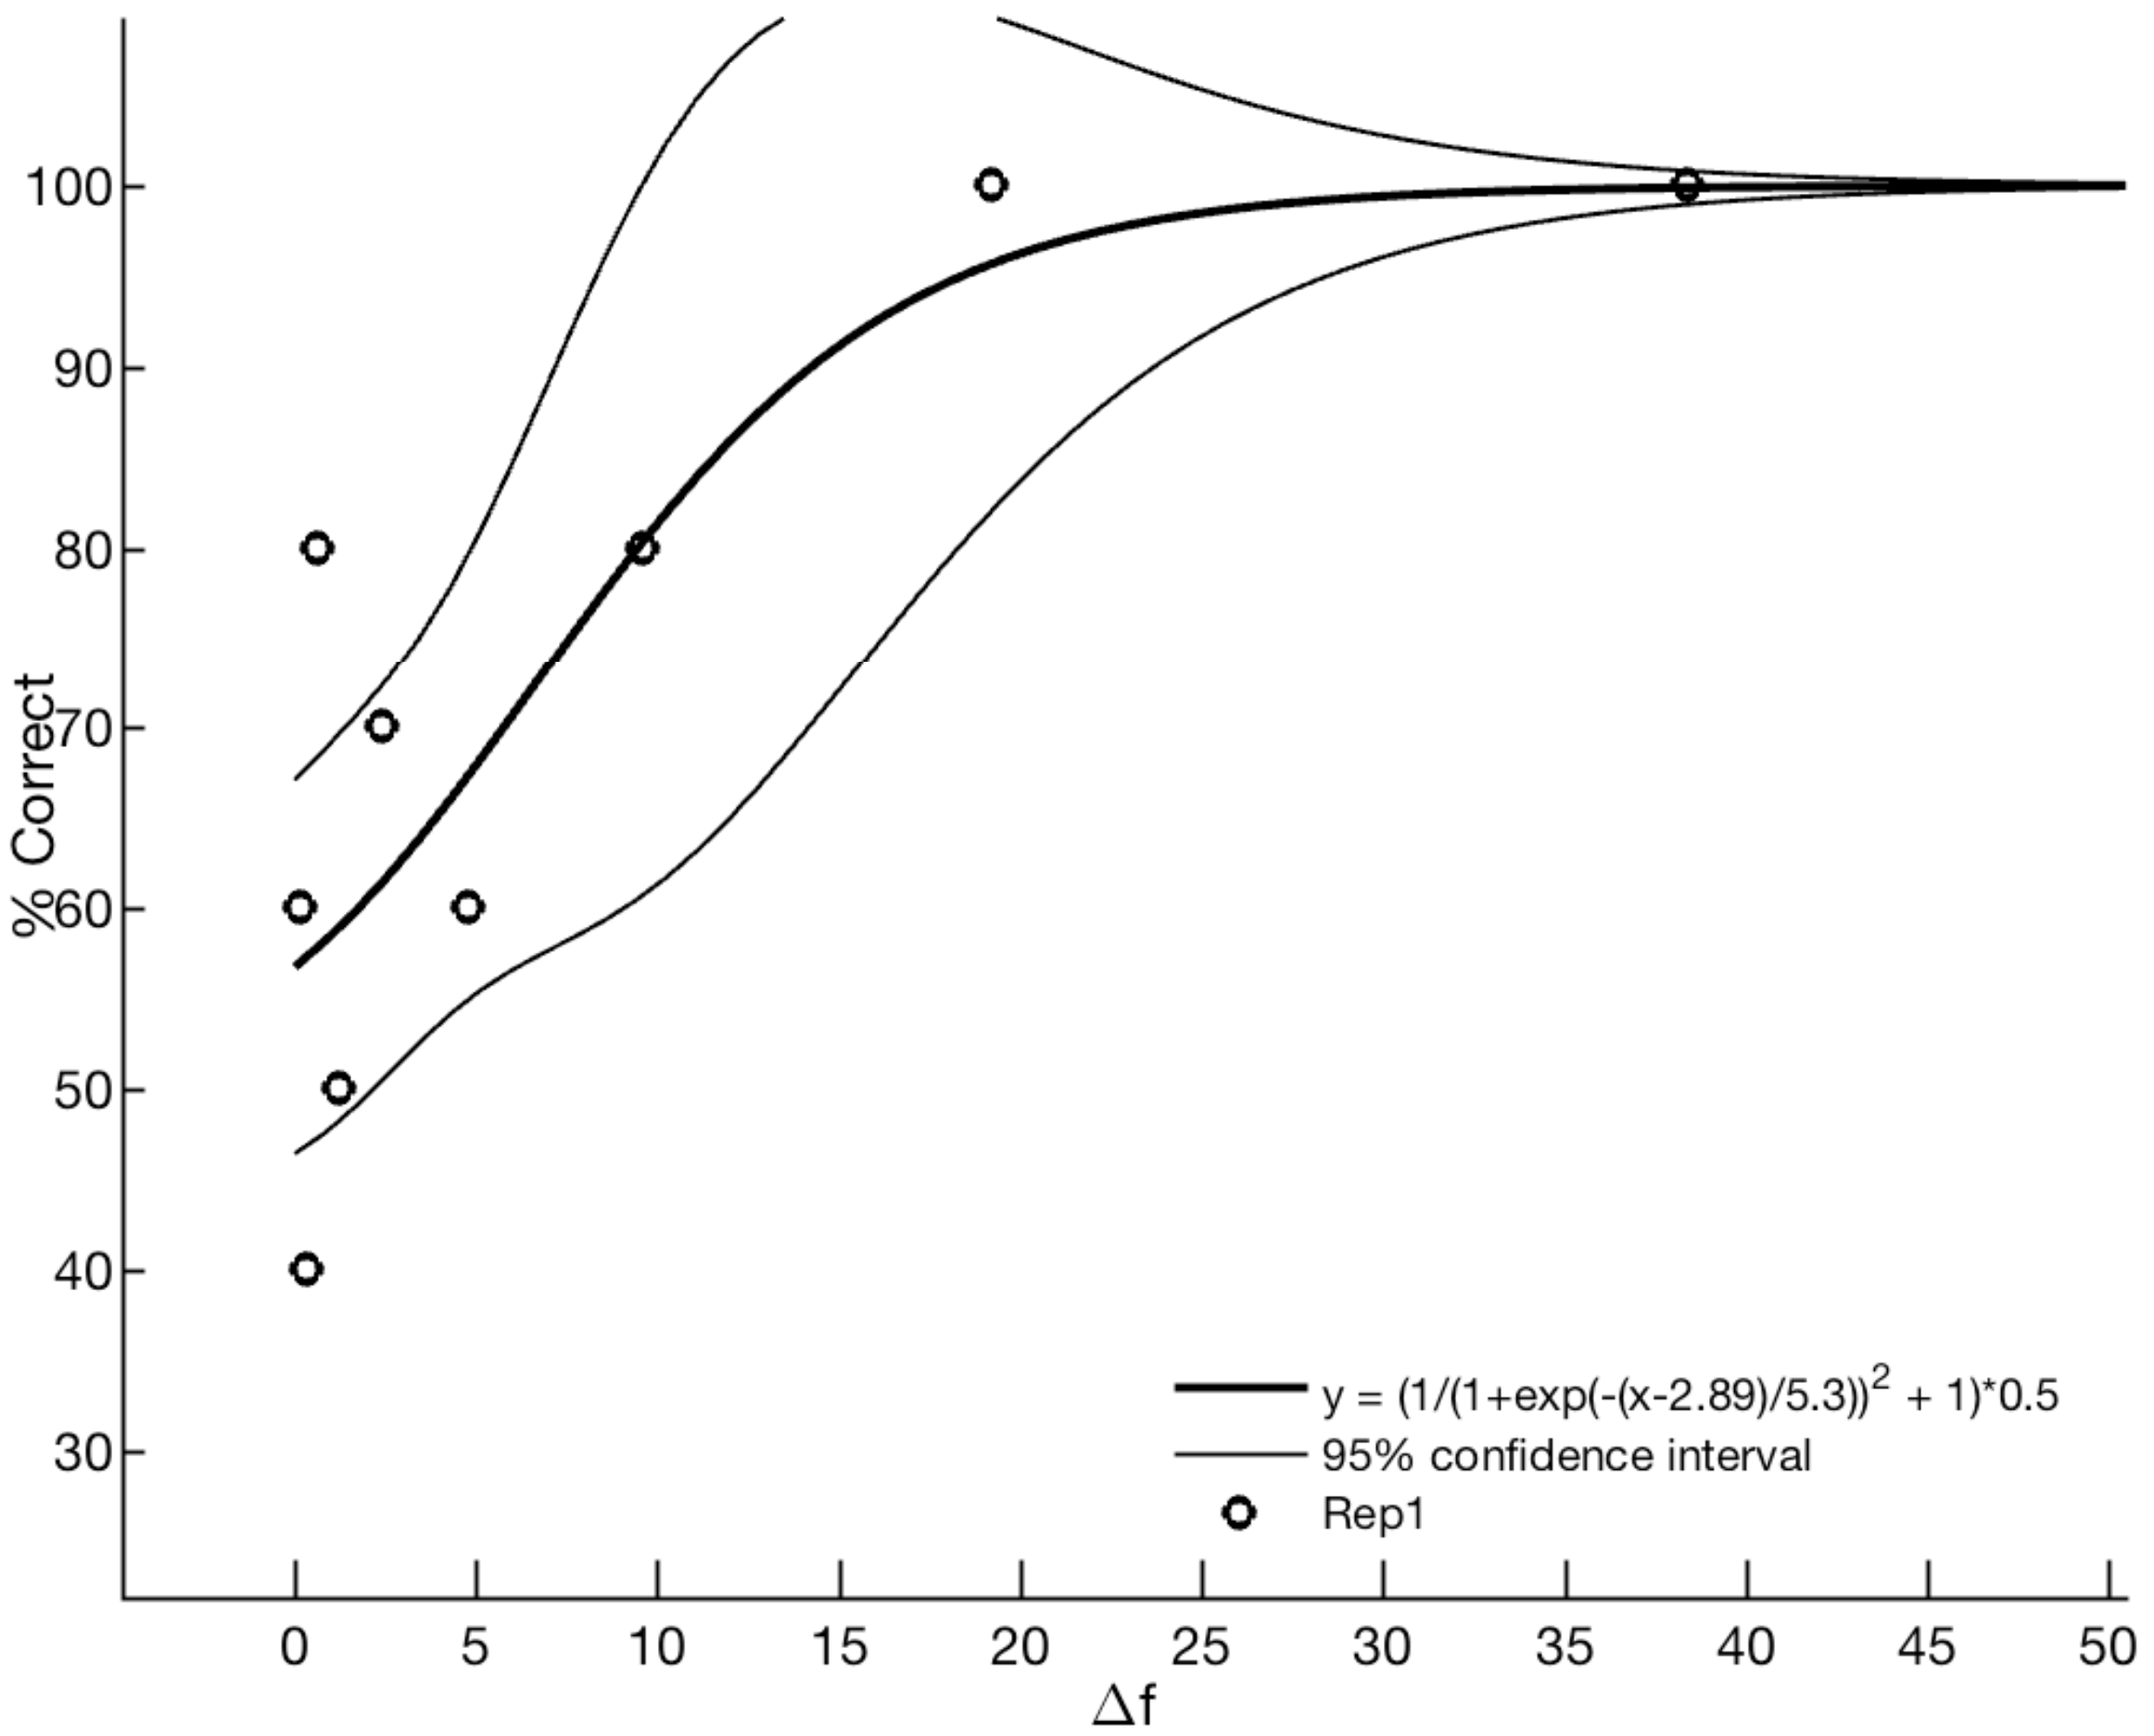
\includegraphics[width = 0.7\textwidth]{Figure/Vores_Figurer/Subject3.png} 
\caption{Raw data and fitted psychometric function for Subject 3.}
\label{fig:Subject3}
\end{figure}
%
\begin{figure}[htb]
\centering
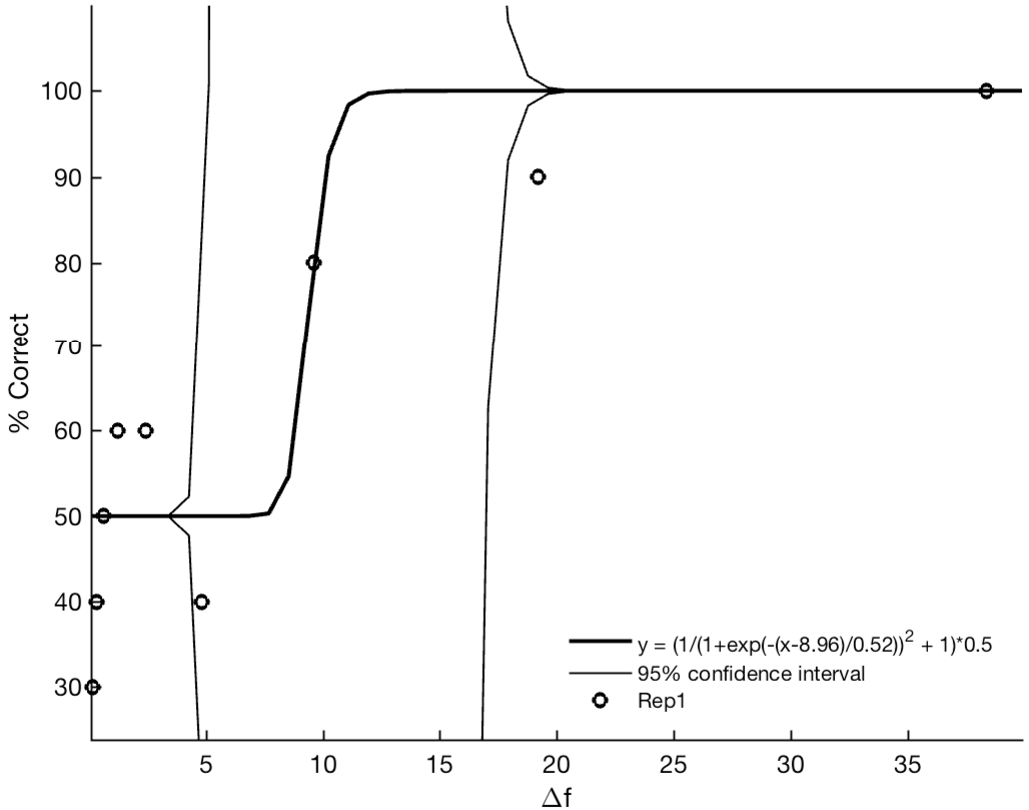
\includegraphics[width = 0.7\textwidth]{Figure/Vores_Figurer/Subject4.png} 
\caption{Raw data and fitted psychometric function for Subject 4.}
\label{fig:Subject4}
\end{figure}
%
\begin{figure}[htb]
\centering
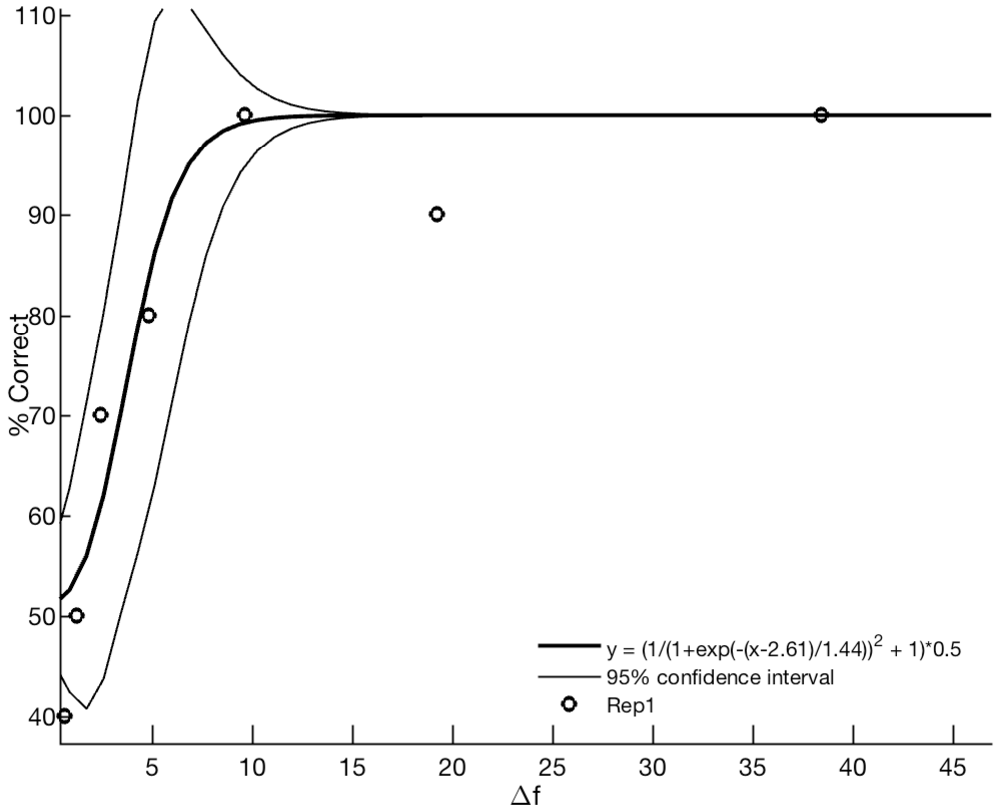
\includegraphics[width = 0.7\textwidth]{Figure/Vores_Figurer/Subject5.png} 
\caption{Raw data and fitted psychometric function for Subject 5.}
\label{fig:Subject5}
\end{figure}

\section*{Analysis}
%
A 2-AFC method is used to collect data which leaves a 50 \% chance of guessing the right answer of the two possibilities. The point for JND is therefore at 75 \%.

From the fitted psychometric function for each subject the JND is read at 75 \% correct answered. In \autoref{tab:JND} the individual test subjects JND are presented along with a calculated mean JND which is 5.31 Hz. 
%
\begin{table}[H]
\centering
\begin{tabular}{l|c}
Subject     & JND ($\Delta$f at 75\%) \\\hline
Subject 1   & 4.40 Hz                 \\\hline
Subject 2   & 1.28 Hz                 \\\hline
Subject 3   & 7.56 Hz                 \\\hline
Subject 4   & 9.42 Hz                 \\\hline
Subject 5   & 3.88 Hz                 \\\hline
mean JND & 5.31 Hz       
\end{tabular}
\caption{JND for all test subjects and mean JND.}
\label{tab:JND}         
\end{table}
\noindent
%
From Webers law the Weber fraction, \textit{k}, can be calculated. According to this sample, the smallest detectable change in pitch perception, \textit{$\Delta$I}, is the mean JND at 5.31 Hz, when compared to the physical stimulus intensity, \textit{I}, of 800 Hz.
% 
\begin{equation}
5.31 Hz = k \cdot 800 Hz \Rightarrow k = \frac{5.31 Hz}{800 Hz} = 0.007
\end{equation}
%
This Weber fraction allows for calculating differential threshold at other intensities, \textit{I}. 
%

\section*{Discussion and conclusion}
%
In the pilot test the female test subjects had problems detecting differences in pitch, especially when the difference between the two frequencies was small, while the male subjects did not experience these problems. This might be due to the fact that one of the male test subjects have more expertise in listening to music and its specific characteristics e.g. when tuning a guitar. Furthermore the subjects might not answer based on the same criterions e.g. they might have different understandings of the word “pitch”. When trying to agree upon a common definition of “pitch”, there might also be different understandings of the words used to describe it.  

From the pilot test it became clear that some of the test subject’s differential threshold was outside the range of the chosen stimuli intensities. Therefore it was decided to expand the intensity range with more frequencies so every test subjects differential threshold would be included. If a test with more subjects had been done, it would likewise have been important to use a frequency range which includes every subject’s differential threshold. Furthermore, a study with more test subjects could be more representative for the true JND.\\[5mm] 
%
Problems with the experimental design could be that the test subjects listens to the tones right after each other. This could be an issue because the subjects easily can compare the first tone of a trial with the last tone of the previously trial, which can influence their responses because they base their answer on memory. Other problems could be the way subjects pressed the A and B button on the computer screen. Some of the subjects used the touch function on the screen while others used the mousepad. For the subjects using the mousepad the mouse on the screen did not move from the chosen button after every comparison and therefore the test subject could be biased to choose the previously pressed button. This issue could have been solved if the subjects after each trial pressed a separate “next” button which will force the subjects to move the cursor to a different position.\\[5mm]
%  
The results shows that the mean JND at 75 \% is 5.31 Hz, which is a bit higher than the expected 1.2 Hz. This might be due to variables affecting the outcome of this study, including ambient noise, distractions and fatigue. If the test was done in an sound isolated lab JND might have been closer to the approximately 1.2 Hz from \citet{Wier1977} findings. Furthermore, \citet{Wier1977} might have used different levels of pitch and more repetitions, which can contribute to different results.\\[5mm] 
%
The calculated Weber fraction should allow for calculating differential threshold at other intensities, \textit{I}. When doing this it is important to be aware of the conditions in which the Weber fraction is calculated. 





 
